%!TEX root = ../paper.tex



\def\AwfyBaseline{%
\begin{knitrout}
\definecolor{shadecolor}{rgb}{0.969, 0.969, 0.969}
% !TEX encoding = UTF-8 Unicode
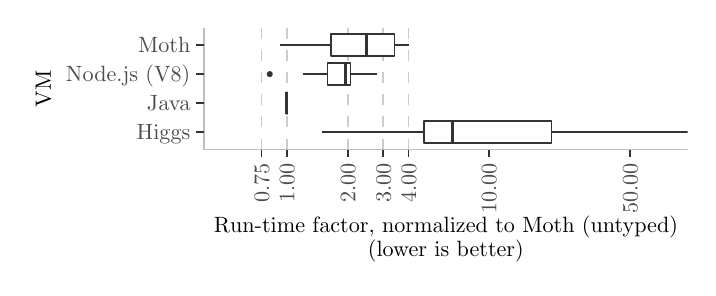
\begin{tikzpicture}[x=1pt,y=1pt]
\definecolor{fillColor}{RGB}{255,255,255}
\path[use as bounding box,fill=fillColor,fill opacity=0.00] (0,0) rectangle (238.49, 86.72);
\begin{scope}
\path[clip] ( 63.73, 42.66) rectangle (238.49, 86.72);
\definecolor{drawColor}{gray}{0.80}

\path[draw=drawColor,line width= 0.6pt,dash pattern=on 4pt off 4pt ,line join=round] ( 84.53, 42.66) -- ( 84.53, 86.72);

\path[draw=drawColor,line width= 0.6pt,dash pattern=on 4pt off 4pt ,line join=round] ( 93.65, 42.66) -- ( 93.65, 86.72);

\path[draw=drawColor,line width= 0.6pt,dash pattern=on 4pt off 4pt ,line join=round] (115.63, 42.66) -- (115.63, 86.72);

\path[draw=drawColor,line width= 0.6pt,dash pattern=on 4pt off 4pt ,line join=round] (128.48, 42.66) -- (128.48, 86.72);

\path[draw=drawColor,line width= 0.6pt,dash pattern=on 4pt off 4pt ,line join=round] (137.61, 42.66) -- (137.61, 86.72);
\definecolor{drawColor}{gray}{0.20}

\path[draw=drawColor,line width= 0.6pt,line join=round] (189.28, 48.96) -- (238.49, 48.96);

\path[draw=drawColor,line width= 0.6pt,line join=round] (143.23, 48.96) -- (106.36, 48.96);
\definecolor{fillColor}{RGB}{255,255,255}

\path[draw=drawColor,line width= 0.6pt,line join=round,line cap=round,fill=fillColor] (189.28, 45.02) --
	(143.23, 45.02) --
	(143.23, 52.89) --
	(189.28, 52.89) --
	(189.28, 45.02) --
	cycle;

\path[draw=drawColor,line width= 1.1pt,line join=round] (153.51, 45.02) -- (153.51, 52.89);

\path[draw=drawColor,line width= 0.6pt,line join=round] ( 93.65, 59.45) -- ( 93.65, 59.45);

\path[draw=drawColor,line width= 0.6pt,line join=round] ( 93.65, 59.45) -- ( 93.65, 59.45);

\path[draw=drawColor,line width= 0.6pt,line join=round,line cap=round,fill=fillColor] ( 93.65, 55.51) --
	( 93.65, 55.51) --
	( 93.65, 63.38) --
	( 93.65, 63.38) --
	( 93.65, 55.51) --
	cycle;

\path[draw=drawColor,line width= 1.1pt,line join=round] ( 93.65, 55.51) -- ( 93.65, 63.38);
\definecolor{fillColor}{gray}{0.20}

\path[draw=drawColor,line width= 0.4pt,line join=round,line cap=round,fill=fillColor] ( 87.48, 69.94) circle (  0.89);

\path[draw=drawColor,line width= 0.6pt,line join=round] (116.67, 69.94) -- (126.23, 69.94);

\path[draw=drawColor,line width= 0.6pt,line join=round] (108.37, 69.94) -- ( 99.31, 69.94);
\definecolor{fillColor}{RGB}{255,255,255}

\path[draw=drawColor,line width= 0.6pt,line join=round,line cap=round,fill=fillColor] (116.67, 66.00) --
	(108.37, 66.00) --
	(108.37, 73.87) --
	(116.67, 73.87) --
	(116.67, 66.00) --
	cycle;

\path[draw=drawColor,line width= 1.1pt,line join=round] (114.97, 66.00) -- (114.97, 73.87);

\path[draw=drawColor,line width= 0.6pt,line join=round] (132.49, 80.43) -- (137.76, 80.43);

\path[draw=drawColor,line width= 0.6pt,line join=round] (109.52, 80.43) -- ( 91.00, 80.43);

\path[draw=drawColor,line width= 0.6pt,line join=round,line cap=round,fill=fillColor] (132.49, 76.50) --
	(109.52, 76.50) --
	(109.52, 84.36) --
	(132.49, 84.36) --
	(132.49, 76.50) --
	cycle;

\path[draw=drawColor,line width= 1.1pt,line join=round] (122.53, 76.50) -- (122.53, 84.36);
\end{scope}
\begin{scope}
\path[clip] (  0.00,  0.00) rectangle (238.49, 86.72);
\definecolor{drawColor}{RGB}{190,190,190}

\path[draw=drawColor,line width= 0.6pt,line join=round] ( 63.73, 42.66) --
	( 63.73, 86.72);
\end{scope}
\begin{scope}
\path[clip] (  0.00,  0.00) rectangle (238.49, 86.72);
\definecolor{drawColor}{gray}{0.30}

\node[text=drawColor,anchor=base east,inner sep=0pt, outer sep=0pt, scale=  0.80] at ( 58.78, 46.20) {Higgs};

\node[text=drawColor,anchor=base east,inner sep=0pt, outer sep=0pt, scale=  0.80] at ( 58.78, 56.69) {Java};

\node[text=drawColor,anchor=base east,inner sep=0pt, outer sep=0pt, scale=  0.80] at ( 58.78, 67.18) {Node.js (V8)};

\node[text=drawColor,anchor=base east,inner sep=0pt, outer sep=0pt, scale=  0.80] at ( 58.78, 77.67) {Moth};
\end{scope}
\begin{scope}
\path[clip] (  0.00,  0.00) rectangle (238.49, 86.72);
\definecolor{drawColor}{gray}{0.20}

\path[draw=drawColor,line width= 0.6pt,line join=round] ( 60.98, 48.96) --
	( 63.73, 48.96);

\path[draw=drawColor,line width= 0.6pt,line join=round] ( 60.98, 59.45) --
	( 63.73, 59.45);

\path[draw=drawColor,line width= 0.6pt,line join=round] ( 60.98, 69.94) --
	( 63.73, 69.94);

\path[draw=drawColor,line width= 0.6pt,line join=round] ( 60.98, 80.43) --
	( 63.73, 80.43);
\end{scope}
\begin{scope}
\path[clip] (  0.00,  0.00) rectangle (238.49, 86.72);
\definecolor{drawColor}{RGB}{190,190,190}

\path[draw=drawColor,line width= 0.6pt,line join=round] ( 63.73, 42.66) --
	(238.49, 42.66);
\end{scope}
\begin{scope}
\path[clip] (  0.00,  0.00) rectangle (238.49, 86.72);
\definecolor{drawColor}{gray}{0.20}

\path[draw=drawColor,line width= 0.6pt,line join=round] ( 84.53, 39.91) --
	( 84.53, 42.66);

\path[draw=drawColor,line width= 0.6pt,line join=round] ( 93.65, 39.91) --
	( 93.65, 42.66);

\path[draw=drawColor,line width= 0.6pt,line join=round] (115.63, 39.91) --
	(115.63, 42.66);

\path[draw=drawColor,line width= 0.6pt,line join=round] (128.48, 39.91) --
	(128.48, 42.66);

\path[draw=drawColor,line width= 0.6pt,line join=round] (137.61, 39.91) --
	(137.61, 42.66);

\path[draw=drawColor,line width= 0.6pt,line join=round] (166.66, 39.91) --
	(166.66, 42.66);

\path[draw=drawColor,line width= 0.6pt,line join=round] (217.69, 39.91) --
	(217.69, 42.66);
\end{scope}
\begin{scope}
\path[clip] (  0.00,  0.00) rectangle (238.49, 86.72);
\definecolor{drawColor}{gray}{0.30}

\node[text=drawColor,rotate= 90.00,anchor=base east,inner sep=0pt, outer sep=0pt, scale=  0.80] at ( 87.28, 37.71) {0.75};

\node[text=drawColor,rotate= 90.00,anchor=base east,inner sep=0pt, outer sep=0pt, scale=  0.80] at ( 96.40, 37.71) {1.00};

\node[text=drawColor,rotate= 90.00,anchor=base east,inner sep=0pt, outer sep=0pt, scale=  0.80] at (118.38, 37.71) {2.00};

\node[text=drawColor,rotate= 90.00,anchor=base east,inner sep=0pt, outer sep=0pt, scale=  0.80] at (131.24, 37.71) {3.00};

\node[text=drawColor,rotate= 90.00,anchor=base east,inner sep=0pt, outer sep=0pt, scale=  0.80] at (140.36, 37.71) {4.00};

\node[text=drawColor,rotate= 90.00,anchor=base east,inner sep=0pt, outer sep=0pt, scale=  0.80] at (169.41, 37.71) {10.00};

\node[text=drawColor,rotate= 90.00,anchor=base east,inner sep=0pt, outer sep=0pt, scale=  0.80] at (220.45, 37.71) {50.00};
\end{scope}
\begin{scope}
\path[clip] (  0.00,  0.00) rectangle (238.49, 86.72);
\definecolor{drawColor}{RGB}{0,0,0}

\node[text=drawColor,anchor=base,inner sep=0pt, outer sep=0pt, scale=  0.80] at (151.11, 12.73) {Run-time factor, normalized to Moth (untyped)};

\node[text=drawColor,anchor=base,inner sep=0pt, outer sep=0pt, scale=  0.80] at (151.11,  4.09) {(lower is better)};
\end{scope}
\begin{scope}
\path[clip] (  0.00,  0.00) rectangle (238.49, 86.72);
\definecolor{drawColor}{RGB}{0,0,0}

\node[text=drawColor,rotate= 90.00,anchor=base,inner sep=0pt, outer sep=0pt, scale=  0.80] at (  8.36, 64.69) {VM};
\end{scope}
\end{tikzpicture}


\end{knitrout}
}%



\newcommand{\OverheadNodeGMeanX}{$1.8$x\xspace}
\newcommand{\OverheadNodeMinX}{$0.8$x\xspace}
\newcommand{\OverheadNodeMaxX}{$2.9$x\xspace}

\newcommand{\OverheadMothGMeanX}{$2.3$x\xspace}
\newcommand{\OverheadMothMinX}{$0.9$x\xspace}
\newcommand{\OverheadMothMaxX}{$4.3$x\xspace}

\newcommand{\OverheadMothNodeGMeanX}{$1.3$x\xspace}
\newcommand{\OverheadMothNodeMinX}{$0.8$x\xspace}
\newcommand{\OverheadMothNodeMaxX}{$2.3$x\xspace}

\newcommand{\OverheadMothNodeGMeanP}{$32$\%\xspace}
\newcommand{\OverheadMothNodeMinP}{$-18$\%\xspace}
\newcommand{\OverheadMothNodeMaxP}{$134$\%\xspace}

\newcommand{\OverheadHiggsGMeanX}{$10.6$x\xspace}
\newcommand{\OverheadHiggsMinX}{$1.5$x\xspace}
\newcommand{\OverheadHiggsMaxX}{$169$x\xspace}


\newcommand{\WarmupCutOff}{$350$\xspace}
